\documentclass[sigconf]{acmart}
\usepackage{ctex}
\usepackage{booktabs} % For formal tables
\usepackage{CJK}
\usepackage{color}
\usepackage{graphicx}
\usepackage{amssymb}
\usepackage{amsmath}
\usepackage{amsthm}
\usepackage{booktabs}
\usepackage{fancyhdr}
\usepackage{extramarks}
\usepackage{amsfonts}
\usepackage{tikz}
\usepackage[plain]{algorithm}
\usepackage{algpseudocode}
\usepackage{listings}


%Conference
\acmConference{Data Communication}{May 2018}{Nanjing, China} 
%\acmYear{2018}
%\copyrightyear{2018}

%\acmPrice{15.00}


\begin{document}

\title{降低移动网页浏览器能耗的技术报告}
%\titlenote{Produces the permission block, and copyright information}
%\subtitle{Extended Abstract}

\author{徐子恒 161160037, 赖伟 161250052}
%\authornote{Note}$  $
%\orcid{1234-5678-9012}
\affiliation{%
  \institution{计算机科学与技术系}
}
\email{161160037@smail.nju.edu.cn,  161250052@smail.nju.edu.cn}

\begin{abstract}

智能手机已经成为了人们生活中必不可少的电子移动设备,但是应用的高能耗导致智能手机的续航始终是一个难以克服的挑战。网页浏览器是智能手机中最核心的应用之一。但因为移动浏览器在性能上进行了大量优化,给移动设备的能源带来了巨大的负担。因此,我们所要介绍的技术正是为了减少智能手机加载网页所消耗的能源,同时尽可能不增加页面加载时间和损害用户体验。

\end{abstract}

\keywords{智能手机; 移动网络浏览器; 网页加载; 能源效率}

\maketitle

\section{Introduction}

网页浏览器是智能手机中最核心的应用之一。但因为移动浏览器在性能上进行了大量优化,给移动设备的能源带来了巨大的负担。因此我们希望提高网页浏览的能效,特别是减少网页加载的能耗。 本文中介绍的技术试图在不影响用户体验且不增加页面加载时间的情况下降低智能手机上网页加载的能耗。

首先,我们会介绍浏览器内部的体系结构和系统行为,以了解能量是如何被用于加载网页,从而发现提高能效的机会。尽管许多浏览器制造商都在努力提高移动设备的能效,但先前的调查结果表明,目前的移动浏览器尚未完全针对网页加载进行能源优化。 首先,不管网络条件如何,网络资源处理总是在积极进行,这就带来了能源效率低下的风险。 其次,渲染率过高,导致大量能量被消耗而没有带来用户可感知的好处。最后,拥有新兴的ARM big.LITTLE架构\cite{3}的现代CPU的节电能力未得到充分利用。 从根本上说,在网页加载过程中过度优化了性能表现,而忽视了能源成本。

为了降低网页加载的能耗,必须重新考虑能源性能的权衡,以制定网页加载的新设计原则。本文会介绍基于这些原则的三种新技术,每种技术对应解决了上述能效问题之一。第一种是使用$network-aware\ resource\ processing$(NRP)技术来适应不断变化的网络条件,从而实现能耗的降低。这种技术使用了自适应资源缓冲技术来动态控制资源下载速度,从而在不增加页面加载时间的情况下提高能源效率。第二种技术是$adaptive\ content\ painting$(ACP)技术,这种技术可以避免不必要的内容渲染,从而达到减少能源开销的目的。并在节能和页面加载时间之间做出权衡来确保用户体验不会受到影响。最后,为了更好地利用big.LITTLE架构,可以使用$application-assisted\ scheduling$(AAS)技术来利用浏览器的内部知识来制定更好的调度决策。具体来说,这种技术采用了基于QoS反馈的自适应线程调度,只要满足相关QoS要求,浏览器就可以让线程在小内核上运行以节约能源。

我们通过修改智能手机上的Chromium浏览器实施了这三项技术。总体而言,这些技术大大降低了网页加载的能源成本。使用美国Alexa排名前100的网站\cite{2}进行的实验评估表明,在使用WiFi的big.LITTLE智能手机上,相比于默认的Chromium浏览器,我们修改后的Chromium浏览器能够实现平均$24.4\%$的系统节能,同时减少$0.3\%$的页面加载时间。在使用3G时,平均系统节能为$22.5\%$,平均页面加载时间增加了$0.41\%$。在另一款没有big.LITTLE支持的智能手机上,我们的技术在使用WiFi时平均可以减少$11.7\%$的能耗。对用户的研究表明,$72\%$的参与者表示愿意在所有情况下使用这些技术,而剩下的$28\%$的用户只愿意在电池电量不足的情况下使用这些技术。

尽管上述实施基于Chromium,但我们提出的技术也可以应用于其他移动浏览器。 Chromium的前两个能源效率问题与Web内容下载,处理和渲染的一般程序有关,所以其他移动浏览器通常会遇到相同的问题别。除Chromium之外,我们还将ACP和AAS技术应用到Firefox,即使没有对Firefox内部的深入了解,也比默认的Firefox平均节省了$10.5\%$的能源。

\section{Background} 

在本节中,我们将介绍Chromium浏览器的体系结构以及加载网页时存在的能源浪费问题。

\subsection{Chromium Browser Architecture}

\begin{figure}[htbp]
	\centering
	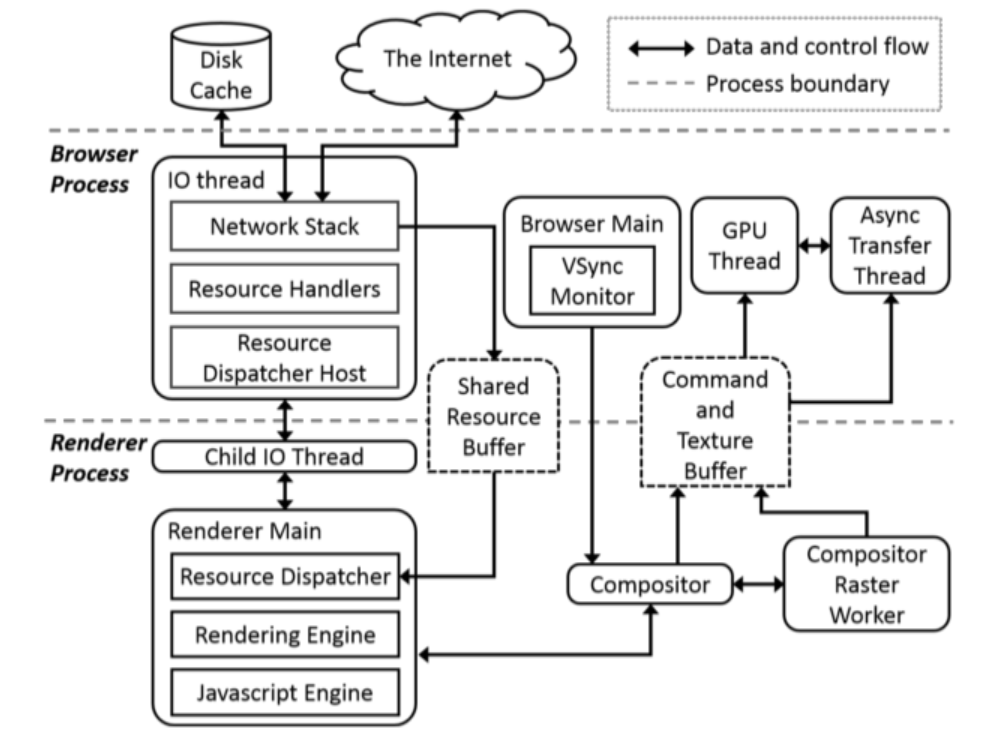
\includegraphics[width=3.4in]{./figure/figure1}
	\caption{Chromium浏览器的体系结构}\label{fig:tasks}
\end{figure}

如图1所示, Chromium使用单个浏览器进程和多个Renderer进程的多进程体系结构。 每个Renderer进程运行一个渲染引擎的实例(以前是WebKit\cite{14},现在是Blink\cite{4})以及解析和执行Web内容的JavaScript引擎。 每个Renderer进程通常对应于Web浏览器UI中的一个选项卡。 浏览器进程运行网络堆栈并从网络中为所有呈现器进程获取网络资源,从而在所有呈现器进程之间共享高效的网络资源。 渲染器进程在沙盒环境中运行,对客户端设备和网络的访问受限,防止渲染引擎中的漏洞侵害整个Web浏览器。

Chromium中的每个进程都有多个线程,。进程和线程被设计为异步工作。浏览器进程和Renderer进程通过IPC机制(例如命名管道)相互通信,并使用共享内存交换数据。浏览器进程将获取的Web资源放入共享资源缓冲区,Renderer进程会从该缓冲区读取数据以创建相应网页的图形层。合成器线程然后将生成的图形数据保存到命令和纹理缓冲区中,以便在浏览器进程中进行GPU处理,因为沙盒渲染器进程没有直接访问GPU的权限。 GPU线程将最终屏幕图像生成到显示帧缓冲区中以显示在设备屏幕上。

图形组成和GPU处理由来自Android框架的称为垂直同步(VSync)的回调驱动。每个VSync信号指示显示帧的开始,以便在下一个VSync之前生成图形数据并将其移动到显示帧缓冲区以供在屏幕上绘制。垂直同步信号每秒产生60次。在浏览器进程中,浏览器主线程的VSync监视器监视VSync信号,并将它们转发到呈现器进程中的合成器线程。

图1所示的体系结构也适用于基于Chromium源代码构建的Google Chrome,Opera Mobile和Android stock 浏览器\cite{6}\cite{19}。浏览器共享相同的渲染引擎,JavaScript引擎和底层核心模块。

\subsection{Energy Cost Of Page Loading}

Web资源处理是浏览的主要组件之一,同时还有资源下载和内容渲染。 Web资源处理通常包括HTML和CSS解析,图像解码,Javascript执行以及更新DOM树和图形层。在Chromium中,只要呈现器进程通知了浏览器进程中可用的数据,就会执行上述处理。如图1所示,这两个进程使用共享资源缓冲区交换数据。浏览器进程在套接字处理程序上使用read系统调用来从网络接收网页资源。每个读取系统调用都会将接收到的数据直接写入资源缓冲区,默认情况下最大数据大小为32 KB。在每次读取系统调用时,无论接收到多少数据,浏览器进程都会立即通知呈现器进程开始处理接收到的数据。

尽管立即处理接收到的数据是很自然的,并且可以最大限度地减少页面加载时间,但这不是节能的。原因在于许多读取系统调用会返回少量数据,从而导致Browser进程和Renderer进程之间的大量IPC。平均而言,每个网页的IPC总数为871(每秒176)。每个IPC都有一个固定的开销。此外,网络资源处理中还有其他开销。每次处理数据块时,即使数据块很小,Renderer进程也必须经历整个数据渲染管道。特别是对于图像数据,Compositor,Raster Worker和Async Transfer线程中涉及许多图形活动。因此,累积的管理费用会浪费大量能源。

加载网页时,Chromium会逐步处理Web资源,并不断将部分渲染的显示结果更新到屏幕上。如图1所示,屏幕更新由VSync信号驱动。在接收到VSync信号后,合成器线程通过共享命令和纹理缓冲区将当前渲染图形数据传送到浏览器进程的GPU线程。 GPU线程然后在GPU上执行特定于平台的图形命令以将所有纹理合成为最终图形结果以显示在屏幕上。这种数据渲染和屏幕更新的图形管道称为内容绘制。

加载网页时可能会出现许多内容,但是在大多数情况下,内容绘制只会在屏幕上产生非常小的甚至不可见的变化。这些无法察觉或非常小的屏幕变化无助于改善用户体验。但是,它们会导致整个图形处理流水线和两个流程之间的IPC发生开销,从而导致不必要的能源成本。


\section{Problem}
问题描述

\section{Overview}
已有工作分类,介绍

\subsection{class 1}
有一些工作从用户的角度 ...



方法结构图,如图 \ref{fig:tasks} 


\subsection{class 2}
还有一些工作从环境的角度 ...

\section{conclusion}
结论

注意:参考文献必须完整


\bibliographystyle{ACM-Reference-Format}
\bibliography{sigproc} 

\end{document}
